\documentclass[a4paper,12pt]{report}

\usepackage{graphicx}
\usepackage{url}
\usepackage{amsmath}
\usepackage[utf8]{inputenc}
\usepackage[english]{babel}
\usepackage[pagestyles]{titlesec}
\usepackage{pgf}
\usepackage{tikz}
\usepackage[section]{placeins}
\usepackage{listings}
\usepackage{color}
\usepackage{seqsplit}
\usepackage{csquotes}

\usetikzlibrary{arrows,automata}
\usetikzlibrary{positioning}

\newpagestyle{mystyle}{
  \sethead{\chaptertitle}{}{}
  \setfoot{}{\thepage}{}}
\pagestyle{mystyle}
 
\setlength{\parindent}{1em}
\setlength{\parskip}{1em}
\graphicspath{ {images/} }

\pagenumbering{roman}

\def\code#1{\texttt{\seqsplit{#1}}}

\definecolor{pblack}{rgb}{0.0,0.0,0.0}
\definecolor{pblue}{rgb}{0.0,0.0,0.5}
\definecolor{pbrightblue}{rgb}{0.0,0.0,1.0}
\definecolor{pgreen}{rgb}{0,0.5,0}
\definecolor{pred}{rgb}{0.9,0,0}
\definecolor{pgrey}{rgb}{0.5,0.5,0.5}
\definecolor{pdarkyellow}{rgb}{0.5,0.5,0.0}
\definecolor{ppurple}{rgb}{0.4,0.05,0.48}

\lstset{
  language            = Java,
  basicstyle          = \scriptsize,
  % xleftmargin         = -4.0em,
  % xrightmargin        = -4.0em,
  frame               = single,
  identifierstyle     = \color{pblack},
  commentstyle        = \color{pgrey},
  keywordstyle        = \color{pblue},
  stringstyle         = \color{pgreen},
  moredelim=[il][\textcolor{pdarkyellow}]{$$},
  moredelim=[is][\textcolor{pdarkyellow}]{\%\%}{\%\%}
}

\newcommand\JSONnumbervaluestyle{\color{pbrightblue}}
\newcommand\JSONstringkeystyle{\color{ppurple}}
\newcommand\JSONstringvaluestyle{\color{pgreen}}

\newif\ifcolonfoundonthisline
\newif\ifsquarebracketopen

\makeatletter

\lstdefinestyle{json}
{
  basicstyle          = \scriptsize,
  % xleftmargin         = -4.0em,
  % xrightmargin        = -4.0em,
  frame               = single,
  showstringspaces    = false,
  keywords            = {false,true},
  alsoletter          = 0123456789.,
  morestring          = [s]{"}{"},
  stringstyle         = \ifcolonfoundonthisline\JSONstringvaluestyle\else\ifsquarebracketopen\JSONstringvaluestyle\else\JSONstringkeystyle\fi\fi,
  MoreSelectCharTable =%
    \lst@DefSaveDef{`:}\colon@json{\processColon@json}
    \lst@DefSaveDef{`[}\squareBracketOpen@json{\processOpenSquareBracket@json}
    \lst@DefSaveDef{`]}\squareBracketClose@json{\processCloseSquareBracket@json},
  keywordstyle        = \color{pblue},
}

\newcommand\processColon@json{%
  \colon@json%
  \ifnum\lst@mode=\lst@Pmode%
    \global\colonfoundonthislinetrue%
  \fi
}

\newcommand\processOpenSquareBracket@json{%
  \squareBracketOpen@json%
  \ifnum\lst@mode=\lst@Pmode%
    \global\squarebracketopentrue%
  \fi
}

\newcommand\processCloseSquareBracket@json{%
  \squareBracketClose@json%
  \ifnum\lst@mode=\lst@Pmode%
    \global\squarebracketopenfalse%
  \fi
}

\lst@AddToHook{Output}{%
  \ifcolonfoundonthisline%
    \ifnum\lst@mode=\lst@Pmode%
      \def\lst@thestyle{\JSONnumbervaluestyle}%
    \fi
  \fi
  %override by keyword style if a keyword is detected!
  \lsthk@DetectKeywords% 
}

% reset the switch at the end of line
\lst@AddToHook{EOL}%
  {\global\colonfoundonthislinefalse}

\makeatother

\begin{document}

% Front matter
\begin{titlepage}
  \begin{center}
    {\LARGE Fast and precise automated analysis of algorithms' time complexity \par}
    \vskip 10.0em
                                                    		
    {\large
      \lineskip 1.0em
      \begin{tabular}[t]{c}
        Dario Simonetti \\Kellogg College\\University of Oxford
      \end{tabular}\par
    }
    \vskip 2.0em
                                                    		
    {\large 3rd of November 2017}
    \vskip 2.0em
                                                    		
    Supervised by: Anthony Widjaja Lin
    \vspace*{\fill}
                                                    		
    {
      \includegraphics[width=5.0em,keepaspectratio]{oxford-logo.png}
      \vskip 1.0em
      A dissertation submitted in partial fulfilment of the requirements for the degree of Master of Science in Software Engineering
    }
  \end{center}
\end{titlepage}

\begin{abstract}
  Profilers have been around in the field of software development since the 70’s
  and have been – and still are – very useful in diagnosing problems and as tools
  for programs optimisation. They can analyse how much time the program is
  spending in each method. Based on this information the developer is able to
  detect what part of the program is taking more time than expected to execute and
  can act to improve it.
          
          
  What profilers can’t do is to estimate how much time it would take when the input
  size is increased. This dissertation supports the development of a tool that will
  estimate the time complexity of an algorithm under test with a high precision. This
  allows accurately estimating the time needed for the algorithm to solve a problem
  for any input size, giving developers a precise idea of how the software will
  behave with input sizes that haven’t been profiled.
\end{abstract}

\vspace*{\fill}
\noindent \textbf{Declaration}

\noindent The author confirms that: this dissertation does not contain material previously submitted for another degree or academic award; and the work presented here is the author's own, except where otherwise stated.

\include{table-of-contents}

\pagenumbering{arabic} % Switch to normal numbers

% Main matter
\chapter{Introduction}

\section{Motivation}
TODO by 02/10
\begin{itemize}
  \item Inaccuracy of Big-O
\end{itemize}


\section{Objectives}
TODO by 02/10

\section{Theory}
TODO by 02/10:
\begin{itemize}
  \item Explain approach principle - measuring time spent each method instead of measuring the whole project for each input of size $n$ and the assumed advantages of using this approach
\end{itemize}

\section{Challenges}
TODO by 02/10:
\begin{itemize}
  \item Explain the challenges that arise by measuring a multitude of methods
\end{itemize}

\chapter{Requirements analysis}

This chapter aims to determine the software requirements to help tailor the software design and implementation. Section \ref{sec:requirementanalysis:definitions} introduces some definitions and concepts that are going to be used across the document. The software can be divided into two different concerns: profiling and analysis. The profiling part is responsible for the measuring of time spent in each instrumented method and its requirements are discussed in Section \ref{sec:requirementanalysis:profiling}. The analysis part takes the data measured by the profiler and works out the time complexity of the algorithm under test. Its requirements are discussed in Section \ref{sec:requirementanalysis:analysis}. These two concerns have very different types of requirements, mainly because the former runs at the same time as the tested algorithm, while the latter does not.

\section{Definitions}
\label{sec:requirementanalysis:definitions}

\subsection{Input size}
Throughout the document, the input size is always indicated with $n$. An algorithm's time complexity quantifies the amount of time taken to run as a function of the input size $n$. For example, for a sorting algorithm the input size $n$ is the size of the list being sorted.

\subsection{Round}
For the scope of this dissertation, a round is the execution of the algorithm under test with a given known input. For example, if the algorithm under test is a sorting algorithm, a round is the sorting of a list of known size $n$.

\subsection{Measurement}
\label{sec:requirementanalysis:definitions:measurement}
Generally speaking, an algorithm is made up of one of more methods, each one keeping the CPU busy for a certain period of time and usually being called several times. For the scope of this dissertation and unless otherwise stated, a measurement captures information about how much time is spent in a specific method and how many times the method is called for a specific input size $n$.

\subsection{Call tree}
A call tree is a more specific version of a call graph\cite{GKM00}, where each node corresponds to a specific stack trace. The difference between a call tree and a call graph is that in the former a method can appear more than once if it's called by different methods, while in the latter it would only appear once and have several edges pointing to it.

\noindent For the scope of this dissertation, three types of call trees are introduced in the next sections.

\subsubsection{Raw call tree}
In a raw call tree, each node contains a measurement for a specific method in a specific call stack path (i.e. tree branch). The measurement is in its raw form, which means that it includes the time spent inside each of the methods it calls (its children). Also, the total times the method has been called is affected by the amount of times its parents have been called. Figure \ref{fig:rawcalltree} shows an example of raw call tree.

\begin{figure}
  \centering
  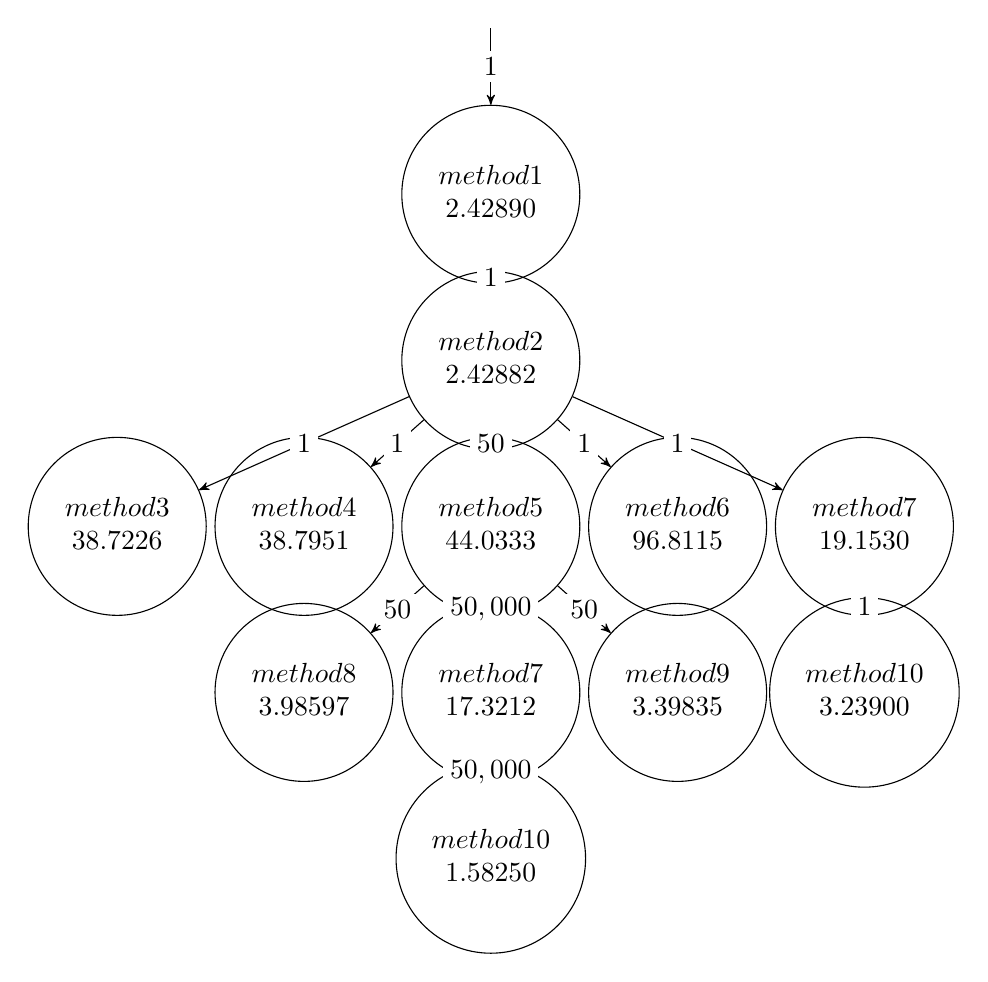
\begin{tikzpicture}[->,>=stealth']
    \coordinate (START);
    
    % FIRST LAYER
    \node[state,
      node distance=6.0em,
    below of=START] (METHOD_1) 
    {
      \begin{tabular}{c}
        $method1$             \\
        \SI{2.42890}{\second} 
      \end{tabular}
    };
    
    
    % SECOND LAYER
    \node[state,
      node distance=6.0em,
    below of=METHOD_1] (METHOD_2) 
    {
      \begin{tabular}{c}
        $method2$             \\
        \SI{2.42882}{\second} 
      \end{tabular}
    };
    
    
    % THIRD LAYER
    \node[state,
      node distance=6.0em,
    below of=METHOD_2] (METHOD_5) 
    {
      \begin{tabular}{c}
        $method5$                   \\
        \SI{44.0333}{\milli\second} 
      \end{tabular}
    };
        
    \node[state,
      node distance=6.75em,
    left of=METHOD_5] (METHOD_4) 
    {
      \begin{tabular}{c}
        $method4$                   \\
        \SI{38.7951}{\milli\second} 
      \end{tabular}
    };
        
    \node[state,
      node distance=6.75em,
    left of=METHOD_4] (METHOD_3) 
    {
      \begin{tabular}{c}
        $method3$                                      \\
        \SI{38.7226}{\milli\second}      \end{tabular} 
        };                                             
                                                       
        \node[state,                                   
        node distance=6.75em,                          
        right of=METHOD_5] (METHOD_6)                  
        {                                              
        \begin{tabular}{c}                             
        $method6$                                      \\
        \SI{96.8115}{\milli\second}                    
      \end{tabular}
    };
        
    \node[state,
      node distance=6.75em,
    right of=METHOD_6] (METHOD_7) 
    {
      \begin{tabular}{c}
        $method7$                   \\
        \SI{19.1530}{\micro\second} 
      \end{tabular}
    };
    
    
    % FOURTH LAYER
    \node[state,
      node distance=6.0em,
    below of=METHOD_5] (METHOD_7B) 
    {
      \begin{tabular}{c}
        $method7$                   \\
        \SI{17.3212}{\micro\second} 
      \end{tabular}
    };
        
    \node[state,
      node distance=6.75em,
    left of=METHOD_7B] (METHOD_8) 
    {
      \begin{tabular}{c}
        $method8$                   \\
        \SI{3.98597}{\milli\second} 
      \end{tabular}
    };
        
    \node[state,
      node distance=6.75em,
    right of=METHOD_7B] (METHOD_9) 
    {
      \begin{tabular}{c}
        $method9$                   \\
        \SI{3.39835}{\milli\second} 
      \end{tabular}
    };
    
    \node[state,
      node distance=6.0em,
    below of=METHOD_7] (METHOD_10) 
    {
      \begin{tabular}{c}
        $method10$                  \\
        \SI{3.23900}{\micro\second} 
      \end{tabular}
    };
    
    
    % FIFTH LAYER
    \node[state,
      node distance=6.0em,
    below of=METHOD_7B] (METHOD_10B) 
    {
      \begin{tabular}{c}
        $method10$                  \\
        \SI{1.58250}{\micro\second} 
      \end{tabular}
    };
    
                
    % LINES
    \begin{scope}[every node/.style={fill=white,inner sep=0.25em,outer sep=0.0em}]
      \path
      (START) edge node {$1$} (METHOD_1)
      (METHOD_1) edge node {$1$} (METHOD_2)
      (METHOD_2) edge node {$1$} (METHOD_3)
      (METHOD_2) edge node {$1$} (METHOD_4)
      (METHOD_2) edge node {$50$} (METHOD_5)
      (METHOD_2) edge node {$1$} (METHOD_6)
      (METHOD_2) edge node {$1$} (METHOD_7)
      (METHOD_5) edge node {$50$} (METHOD_8)
      (METHOD_5) edge node {$50,000$} (METHOD_7B)
      (METHOD_5) edge node {$50$} (METHOD_9)
      (METHOD_7) edge node {$1$} (METHOD_10)
      (METHOD_7B) edge node {$50,000$} (METHOD_10B)
      ;
    \end{scope}
  \end{tikzpicture}
  \caption{A raw call tree}
  \label{fig:rawcalltree}
\end{figure}

\noindent Note: when displayed graphically in this document, the number shown in the node is the average time spent in the method (worked out dividing the total time by the number of calls), while the number shown in the edge is the number of times the method has been called. Also note that values are always approximated to 6 significant digits. This is true for normalised call trees too.


\subsubsection{Normalised call tree}
In a normalised call tree, each node only contains data related to that specific method in isolation of other nodes in the tree. Each node then contains information about how much time has been spent inside this method, excluding the time spent in each of its children. The number of times the method has been called only includes the number of times it has been called directly. Figure \ref{fig:normalisedcalltree} is the normalised version of Figure \ref{fig:rawcalltree}. Note that given a tree representation like this, it's not always possible to determine whether it is a raw or normalised call tree. Call trees in this document are always normalised unless otherwise stated.

\begin{figure}
  \centering
  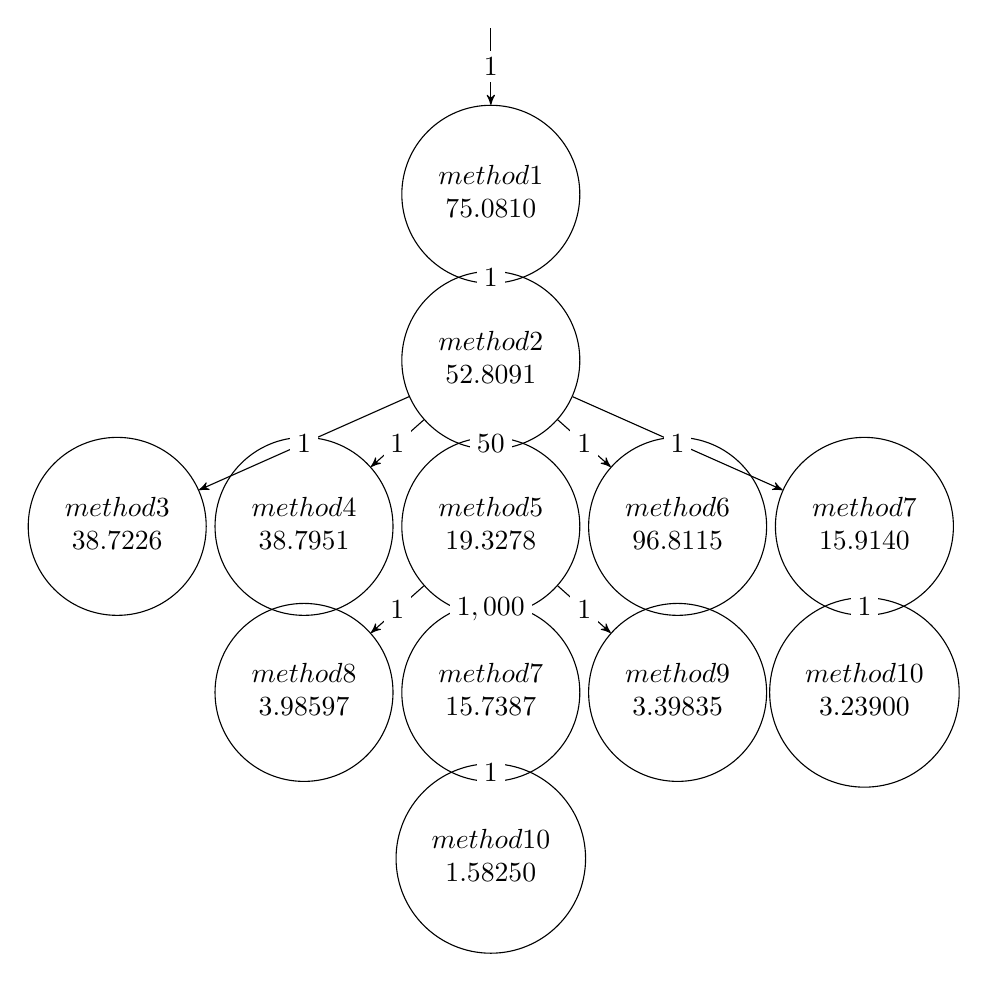
\begin{tikzpicture}[->,>=stealth']
    \coordinate (START);
    
    % FIRST LAYER
    \node[state,
      node distance=6.0em,
    below of=START] (METHOD_1) 
    {
      \begin{tabular}{c}
        $method1$                   \\
        \SI{75.0810}{\micro\second} 
      \end{tabular}
    };
    
    
    % SECOND LAYER
    \node[state,
      node distance=6.0em,
    below of=METHOD_1] (METHOD_2) 
    {
      \begin{tabular}{c}
        $method2$                   \\
        \SI{52.8091}{\milli\second} 
      \end{tabular}
    };
    
    
    % THIRD LAYER
    \node[state,
      node distance=6.0em,
    below of=METHOD_2] (METHOD_5) 
    {
      \begin{tabular}{c}
        $method5$                   \\
        \SI{19.3278}{\milli\second} 
      \end{tabular}
    };
        
    \node[state,
      node distance=6.75em,
    left of=METHOD_5] (METHOD_4) 
    {
      \begin{tabular}{c}
        $method4$                   \\
        \SI{38.7951}{\milli\second} 
      \end{tabular}
    };
        
    \node[state,
      node distance=6.75em,
    left of=METHOD_4] (METHOD_3) 
    {
      \begin{tabular}{c}
        $method3$                   \\
        \SI{38.7226}{\milli\second} 
      \end{tabular}
    };
        
    \node[state,
      node distance=6.75em,
    right of=METHOD_5] (METHOD_6) 
    {
      \begin{tabular}{c}
        $method6$                   \\
        \SI{96.8115}{\milli\second} 
      \end{tabular}
    };
        
    \node[state,
      node distance=6.75em,
    right of=METHOD_6] (METHOD_7) 
    {
      \begin{tabular}{c}
        $method7$                   \\
        \SI{15.9140}{\micro\second} 
      \end{tabular}
    };
    
    
    % FOURTH LAYER
    \node[state,
      node distance=6.0em,
    below of=METHOD_5] (METHOD_7B) 
    {
      \begin{tabular}{c}
        $method7$                   \\
        \SI{15.7387}{\micro\second} 
      \end{tabular}
    };
        
    \node[state,
      node distance=6.75em,
    left of=METHOD_7B] (METHOD_8) 
    {
      \begin{tabular}{c}
        $method8$                   \\
        \SI{3.98597}{\milli\second} 
      \end{tabular}
    };
        
    \node[state,
      node distance=6.75em,
    right of=METHOD_7B] (METHOD_9) 
    {
      \begin{tabular}{c}
        $method9$                   \\
        \SI{3.39835}{\milli\second} 
      \end{tabular}
    };
    
    \node[state,
      node distance=6.0em,
    below of=METHOD_7] (METHOD_10) 
    {
      \begin{tabular}{c}
        $method10$                  \\
        \SI{3.23900}{\micro\second} 
      \end{tabular}
    };
    
    
    % FIFTH LAYER
    \node[state,
      node distance=6.0em,
    below of=METHOD_7B] (METHOD_10B) 
    {
      \begin{tabular}{c}
        $method10$                  \\
        \SI{1.58250}{\micro\second} 
      \end{tabular}
    };
    
                
    % LINES
    \begin{scope}[every node/.style={fill=white,inner sep=0.25em,outer sep=0.0em}]
      \path
      (START) edge node {$1$} (METHOD_1)
      (METHOD_1) edge node {$1$} (METHOD_2)
      (METHOD_2) edge node {$1$} (METHOD_3)
      (METHOD_2) edge node {$1$} (METHOD_4)
      (METHOD_2) edge node {$50$} (METHOD_5)
      (METHOD_2) edge node {$1$} (METHOD_6)
      (METHOD_2) edge node {$1$} (METHOD_7)
      (METHOD_5) edge node {$1$} (METHOD_8)
      (METHOD_5) edge node {$1,000$} (METHOD_7B)
      (METHOD_5) edge node {$1$} (METHOD_9)
      (METHOD_7) edge node {$1$} (METHOD_10)
      (METHOD_7B) edge node {$1$} (METHOD_10B)
      ;
    \end{scope}
  \end{tikzpicture}
  \caption{A normalised call tree}
  \label{fig:normalisedcalltree}
\end{figure}

\subsubsection{Interpolated call tree}
An interpolated call tree represents a normalised tree as a function of $n$. Each node contains information about the amount of time the method takes to run and the number of times the method is called as a function of the input size $n$. An interpolated call tree is a way of accurately describing an algorithm's time complexity. For example, the interpolated call tree in Figure \ref{fig:interpolatedcalltree} describes an algorithm with time complexity $1 \cdot (2n + ((n^2 + 2) \cdot (n^3 + 0.5 \cdot n)) + (log(3n) \cdot (2.7 \cdot n \cdot log(n) + 4))$.

\begin{figure}
  \centering
  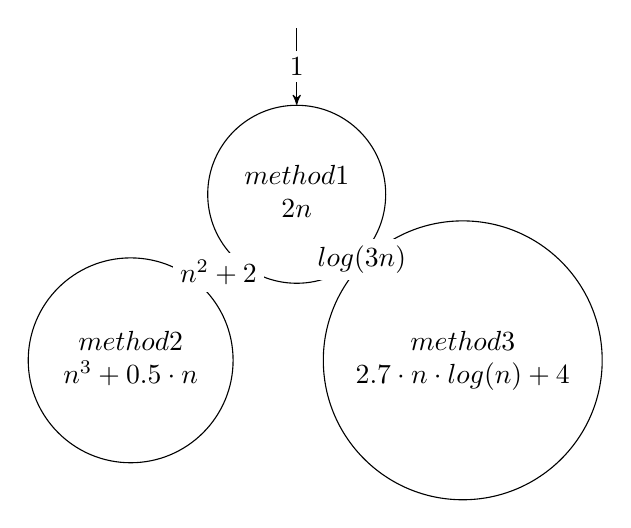
\begin{tikzpicture}[->,>=stealth']
    \coordinate (START);
    
    % FIRST LAYER
    \node[state,
      node distance=6.0em,
    below of=START] (METHOD_1) 
    {
      \begin{tabular}{c}
        $method1$ \\
        $2n$      
      \end{tabular}
    };
    
    
    % SECOND LAYER
    \node[state,
      node distance=6.0em,
      below of=METHOD_1,
    xshift=-6.0em] (METHOD_2) 
    {
      \begin{tabular}{c}
        $method2$           \\
        $n^3 + 0.5 \cdot n$ 
      \end{tabular}
    };
    \node[state,
      node distance=6.0em,
      below of=METHOD_1,
    xshift=6.0em] (METHOD_3) 
    {
      \begin{tabular}{c}
        $method3$                      \\
        $2.7 \cdot n \cdot log(n) + 4$ 
      \end{tabular}
    };
    
                
    % LINES
    \begin{scope}[every node/.style={fill=white,inner sep=0.25em,outer sep=0.0em}]
      \path
      (START) edge node {$1$} (METHOD_1)
      (METHOD_1) edge node {$n^2 + 2$} (METHOD_2)
      (METHOD_1) edge node {$log(3n)$} (METHOD_3)
      ;
    \end{scope}
  \end{tikzpicture}
  \caption{An interpolated call tree}
  \label{fig:interpolatedcalltree}
\end{figure}




\section{Profiling}
\label{sec:requirementanalysis:profiling}

\subsection{Limited observer effect impact}
As the profiler runs together with the algorithm under test, extra care needs to be taken in order to not be impacted by the observer effect \cite{MSH08}. Because they are sharing the same CPU it is not possible to avoid the observer effect, but several things can be done in order to limit its impact as well as measuring it.

\subsection{Manual methods selection}
Often there are methods that are called very frequently and are very quick (e.g. getters and setters) and for this reason there needs to be a way of specifying which methods should be profiled and which ones should not.

\noindent It should also allow to profile 3rd party code as it is sometimes useful to see when a lot of time is spent in a library that there is no control over, so that it can be potentially be swapped out for a different, or a custom-built one. This will also allow to profile and analyse code that is part of the Java SDK, such as sorting and searching algorithms.

\noindent Method selection should be possible via Java annotations in the algorithm under test, as well as by specifying whitelists and blacklists of methods' fully qualified names.

\subsection{Storage}
The profiler needs to be able to handle and store a vast number of measurements without running out of memory and space on disk.

\subsection{Concurrency}
\label{sec:requirementanalysis:profiling:concurrency}
The profiler must only support single-threaded algorithms.

\noindent TODO by 25/09: more?

\section{Analysis}
\label{sec:requirementanalysis:analysis}

\subsection{Custom test}
As the software does not perform any static analysis of the algorithm under test, it does not know how to make sure to test all of the edge cases. Moreover, it does not know whether the edge cases are an important factor for the user who is analysing the algorithm (end user). For example, when measuring a sorting algorithm it might be important for the end user to know how well it performs under specific circumstances, such as when the list is already ordered or ordered in decreasing order; it might be completely irrelevant too.

\noindent For these reasons, the test that is run by the profiler for each \emph{n} must be defined by the end user.

\subsection{Configuration}
It needs to be possible to easily change the analysis configuration in order to find the right balance between speed and accuracy:
\begin{itemize}
  \item \textbf{Max \emph{n}}: maximum value of \emph{n} to test the algorithm with
  \item \textbf{Number of samples per round}: number of samples to collect between $n = 1$ and $n = maxN$
  \item \textbf{Samples distribution}: how to distribute the samples in each round (linearly or exponentially)
  \item \textbf{Number of rounds per \emph{n}}: number of times to test the algorithm for each \emph{n}
  \item \textbf{Number of warmup rounds per \emph{n}}: number of times to run the algorithm without profiling for each \emph{n}
  \item \textbf{Number of max outliers to exclude}: maximum number of out outliers to remove for each \emph{n}
\end{itemize}

\subsection{Supported curves}
Because the software analyses the methods in isolation, it only needs to fit the measured data to one of the basic \enquote{primitives}:
\begin{itemize}
  \item Constant ($f(n) = a$)
  \item Linear ($f(n) = a \cdot n + b$)
  \item Quadratic ($f(n) = a \cdot n^2 + b \cdot n + c$)
  \item Cubic ($f(n) = a \cdot n^3 + b \cdot n^2 + c \cdot n + d$)
  \item Logarithmic ($f(n) = a \cdot log(n) + b$)
  \item Linearithmic ($f(n) = a \cdot n \cdot log(n) + b$)
  \item Exponential ($f(n) = a \cdot e^{(n \cdot b)} + c$)
\end{itemize}


\noindent TODO by 25/09: more?
\chapter{Design}

The purpose of this chapter is to describe how the software is designed based on the requirements specified in the previous chapter. Section \ref{sec:design:overview} gives a design overview and introduce the concept of module and the motivations for adopting this structure. Sections \ref{sec:design:annotations}-\ref{sec:design:timecomplexityanalyser} will each describe one of the modules that make up the whole software.

% TODO: why Java? Comfortable with it, easy instrumentation, generics, Akka, compatible with Scala (maybe not in this chapter)

\section{Overview}
\label{sec:design:overview}
The software will take a dynamic approach to determine the time complexity of the algorithm under test. The algorithm will be run with inputs of different size $n$, while at the same time recording how long is spent in each measured method and how many times each measured method is called.

\noindent Only the methods the end user thinks are relevant are measured and for each one of them their time complexity is calculated. The reasoning behind this is that measuring the time complexity method by method is more accurate than measuring the whole algorithm's while also not increasing the time needed for the dynamic analysis. It's then trivial to work out the time complexity of the whole algorithm based on the time complexity of the measured methods that compose it.

\noindent In order to ensure low coupling and high cohesion \cite{EYC79}, the software will be divided in different modules, each one with a different responsibility. Classes within each module will honour the same principles. This will bring several advantages:
\begin{itemize}
  \item \textbf{Encouraged refactoring}: modules and classes can be refactored and optimised without impacting the rest of the code. This will encourage perfecting the code to keep it clean and maintainable
  \item \textbf{Increased reusability}: as each module and class is built to only do one job well (Single Responsibility Principle \cite{RCM03}), it is easy to reuse it for different applications
  \item \textbf{Improved robustness}: when the cohesion is high the code complexity is much lower, making it much easier to test
  \item \textbf{Reduced code duplication}: instead of defining logic more than once, it is coded once and used several time across the product (Don't Repeat Yourself \cite{AHT99}). Any changes in the logic would only have to be implemented in one single place
\end{itemize}

\noindent Figure \ref{fig:modules} shows an overview of the modules and the dependencies within them. The next chapters describe the modules shown in the diagram.

\begin{figure}
  \centering
  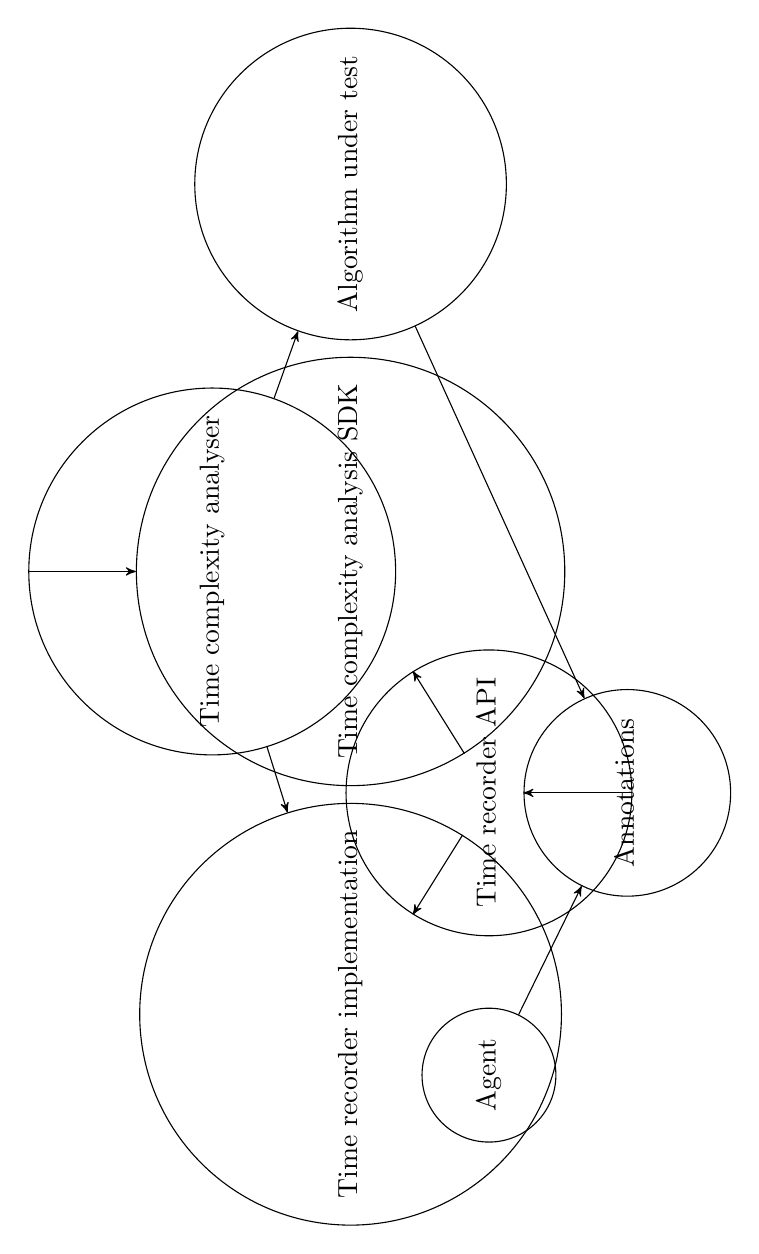
\begin{tikzpicture}[->,>=stealth', rotate=90, transform shape]
    % FIRST LAYER
    \node[state] (TIME_COMPLEXITY_ANALYSER) 
    {
      \begin{tabular}{c}
        Time complexity analyser 
      \end{tabular}
    };
              
    % SECOND LAYER
    \node[state,
      node distance=5.0em,
      below of=TIME_COMPLEXITY_ANALYSER] (TIME_COMPLEXITY_ANALYSIS_SDK) 
    {
      \begin{tabular}{c}
        Time complexity analysis SDK 
      \end{tabular}
    };
              
    \node[state,
      node distance=14.0em,
      left of=TIME_COMPLEXITY_ANALYSIS_SDK,
      xshift=-2.0em] (TIME_RECORDER_IMPL) 
    {
      \begin{tabular}{c}
        Time recorder implementation 
      \end{tabular}
    };
              
    \node[state,
      node distance=14.0em,
      right of=TIME_COMPLEXITY_ANALYSIS_SDK] (TEST_ALGORITHM) 
    {
      \begin{tabular}{c}
        Algorithm under test 
      \end{tabular}
    };
              
    % THIRD LAYER
    \node[state,
      node distance=5.0em,
      below of=TIME_RECORDER_IMPL,
      xshift=-2.2em] (AGENT) 
    {
      \begin{tabular}{c}
        Agent 
      \end{tabular}
    };
            
    \node[state,
      node distance=5.0em,
      below of=TIME_RECORDER_IMPL,
      xshift=+8.0em] (TIME_RECORDER_API) 
    {
      \begin{tabular}{c}
        Time recorder API 
      \end{tabular}
    };
              
    % FOURTH LAYER
    \node[state,
      node distance=5.0em,
      below of=TIME_RECORDER_API] (ANNOTATIONS) 
    {
      \begin{tabular}{c}
        Annotations 
      \end{tabular}
    };
            
    % LINES
    \path 
    (TIME_COMPLEXITY_ANALYSER) edge (TIME_RECORDER_IMPL)
    (TIME_COMPLEXITY_ANALYSER) edge (TIME_COMPLEXITY_ANALYSIS_SDK)
    (TIME_COMPLEXITY_ANALYSER) edge (TEST_ALGORITHM)
    (TIME_RECORDER_IMPL) edge (TIME_RECORDER_API)
    (TIME_COMPLEXITY_ANALYSIS_SDK) edge (TIME_RECORDER_API)
    (TEST_ALGORITHM) edge (ANNOTATIONS)
    (TIME_RECORDER_API) edge (ANNOTATIONS)
    (AGENT) edge (ANNOTATIONS)
    ;
  \end{tikzpicture}
  \caption{Modules overview}
  \label{fig:modules}
\end{figure}

\section{Annotations}
\label{sec:design:annotations}
This module doesn't contain any implementation, only Java annotations. A Java annotation is a special syntax used to associate metadata to packages, classes, methods, parameters and variables. They can be read and interpreted by the compiler at compile time or by an agent at runtime. These annotations are used to inform the agent (see next section) about what methods to instrument and measure.


\section{Agent}
\label{sec:design:agent}
This module contains the logic to instrument the algorithm under test. First the agent will detect which methods need to be instrumented based on annotations, whitelists and blacklists. Secondly the agent will instrument each of these methods by measuring the time passed during the method execution. This number will then be passed to the time recorder implementation (see next sections) which will take care of storing it for later processing.

\noindent The built agent is a JAR\footnote{https://docs.oracle.com/javase/8/docs/technotes/guides/jar/jarGuide.html} file which will need to be attached to the system by passing \code{-javaagent:jarpath[=options]}\footnote{https://docs.oracle.com/javase/8/docs/api/java/lang/instrument/package-summary.html} on the command-line, where \code{jarpath} is the path to the agent JAR while \code{options} are the options, such as whitelists and blacklists. This will instrument the algorithm under test at runtime when the instrumented methods are used for the first time.


\section{Time recorder API}
This module defines the API needed for time recording. The API will need to provide the interface for three different features:
\begin{itemize}
  \item \textbf{Start}: used by the system just before the algorithm's time complexity is about to be measured. This will reset any existing data in the time recorder implementation and start a fresh new recording
  \item \textbf{Report time}: used by the agent when an instrumented has just finished running to inform the time recorder implementation about how long it took. The implementation will take care of storing this information for later processing
  \item \textbf{Stop}: used by the system just after the algorithm is done running. This will shut down the time recorder implementation and return all the recorded data
\end{itemize}

\noindent The recorded data is returned in form of a raw call tree. Each node in the tree has an associated measurement. For the context of this dissertation, a measurement consists of how long is spent in a method and how many times the method is called.

\noindent Defining an API for time recording will keep the interface separated from the implementation so that the whole system works without needing to know the inner workings of the time recorder implementation. This allows easily swapping and comparing different implementations, which will be very useful in order to fine-tune them. On top of that developers can easily attempt building their own implementation in order to improve the existing one or to fine tune it for their specific use case. Because the implementation is probably the most delicate part of the whole system (as it needs to be accurate while ensuring a limited observer effect), being able to change the implementation must be an easy task.

\section{Time recorder implementation}
This module implements the time recorder API described in the previous section. The implementation needs to ensure that the act of recording doesn't have an impact on the actual measurement of the algorithm under test (i.e. limited observer effect). Time recording is purposely kept separate from the time complexity analysis as the former is run together with the algorithm under test while the latter isn't. In order to limit the observer effect is then essential to keep the CPU load as low as possible while the algorithm under test is running. 

\noindent This implementation is only responsible for storing the measured data for later retrieval and processing, which is something that doesn't put a big workload on the CPU. Had the time complexity be analysised as the algorithm under test was running, the measured time complexity would likely be far less accurate as the analysis is computationally expensive (see next sections).

\section{Time complexity analysis SDK}
This module is responsible for analysing the data captured by the time recorder. It does so in 7 different steps:
\begin{enumerate}
  \item \textbf{Warm-up}: run some rounds and ignore the recorded data. This will instrument all the methods that need to be measured, which will make the algorithm under test run slightly slower. The end user will be able to choose how many warm-up rounds to have (could be zero)
  \item \textbf{Record}: run the recording rounds. The rounds are run with different $n$ and each will produce a call tree measured by the time recorder. The end user will be able to choose what $n$'s to use and how many rounds to run for each $n$
  \item \textbf{Aggregate}: for each $n$ there are now several call trees. The aggregation will, for each $n$, take the set of call trees and transform it into one single call tree, where each node in it contains the associated set of measurements
  \item \textbf{Clean up and average}: there are now several measurements in each node in each call tree, some of which are far from the average for that node (outliers) and can be removed. The remaining measurements in each node are averaged together so that there is only one value per node in each call tree. The end user will be able to choose the upper limit of how many outliers to exclude (could be zero)
  \item \textbf{Normalise}: each node in the call tree now contains information about how many times it has been called and how much total time has been spent inside that method. Because of the simple nature of the time recorder, each node is affected by other nodes in the same branch. The number of times it has been called is affected by the number of times its parent has been called while the time spent inside the method is affected by the time spent in its children too. The normalisation process takes the call tree in raw format (see Figure \ref{fig:rawcalltree}) and ensures that each node only contains data related to that specific node (see Figure \ref{fig:normalisedcalltree})
  \item \textbf{Interpolate}: there is now a normalised call tree for each $n$ with one measurement per node. For each node in a call tree, the same node can be found in another call tree that is associated to a different $n$, simply by following the same path in the trees. Interpolation is the act of finding a curve that best approximates the relationship between these nodes across different call trees, i.e. a function $f(n)$ that takes $n$ as input and returns the measurement as output (see example in Figure \ref{fig:interpolatedcalltree}). This function accurately describes the time complexity of the corresponding method
  \item \textbf{Calculate time complexity}: there is now one single call tree with a function $f(n)$ per node approximating the measurement of the corresponding method as a function of $n$. The time complexity can be calculated, describing the whole algorithm as a function of $n$ by simply navigating through the tree
\end{enumerate}

\noindent Once the time complexity function is determined, accurately calculating how long the algorithm would take to run given an input size $n$ can be done in constant time as it's a simple calculation.

\noindent Being an SDK, this module provides the tools for performing the analysis of an algorithm but won't do any of the above until correctly configured. For this reason this module has  has no dependency on the time recorder implementation and instead the code is done against the time recorder API. The time recorder implementation will be supplied at runtime and the whole wiring will be done by the time complexity analyser module (see next sections). Also it has no dependency on the algorithm under test and instead defines an interface describing an algorithm, which the algorithm under test will implement at runtime (see next chapter).

\noindent The SDK parameters specified above allow the end user to tweak the analysis to favour accuracy over speed and vice versa. The more rounds are run and the more accurate the time complexity will be and the slower it will be to calculate it.

\section{Algorithm under test}
This is the algorithm that is under test and that will be analysed. It can have a dependency on the annotations module, in case it wants to specify what methods to measure by using the provided annotations.

\section{Time complexity analyser}
\label{sec:design:timecomplexityanalyser}
This module puts everything together. It takes the time recording implementation and the algorithm under test and then uses the time complexity analysis SDK to calculate the algorithm's time complexity. This is where the end user can tweak the analysis by changing what SDK parameters and what time recorder implementation to use (and with what parameters, if there are any).
\chapter{Implementation}

This chapter discusses how the software has been implemented. Section \ref{sec:implementation:overview} gives an overview about the tools and techniques being used. Sections \ref{sec:implementation:annotations}-\ref{sec:implementation:timecomplexityanalyser} will discuss the implementation of each existing module that has been introduced in the previous chapter.

\section{Overview}
\label{sec:implementation:overview}

\subsection{Important considerations}
As mentioned in previous chapters, one of the most important aspects of the product is to limit the observer effect. It is extremely important that the act of instrumenting and analysing the algorithm under test has the smallest possible impact on the algorithm's performance. Performance in programs that run on the JVM is also impacted be the garbage collection, given that when that happens all the threads are temporarily paused. This means that the act of collecting measurements must not have a big impact on memory, or the garbage collection will happen too often having a great impact on the algorithm's performance.

\noindent Considering this, it would be very hard, if not impossible, to come up with the theory supporting the instrumentation and measuring logic. Instead, different implementations will be attempted, discussed and compared in the following sections. All the different approaches will of course keep performance and memory usage in mind.

\subsection{Modules and dependencies}
The modules discussed in the previous chapters are defined as Maven\footnote{\url{https://maven.apache.org/}} modules. Maven is a tool that can be used to build and manage Java-based projects. Modules can be defined via a \code{pom.xml} file in the module's root folder, specifying the module group ID, artifact ID, version and the dependencies it has on other Maven modules. Maven dependencies could be defined by the user or could be 3rd party modules that exist in Maven public repositories. An example of a \code{pom.xml} file can be find in Appendix \ref{sec:appendices:examplepomfile}.

\subsection{Testing}
The concept of test-driven development (TDD) is applied to all modules. Tests that describe requirements are written prior to the implementation, then the implementation is added ensuring that the tests pass. This process inspires confidence, makes the software more robust and allows for easy refactoring. On top of that, benchmarks are used across modules that are performance-critical, ensuring the CPU time they use is minimal.

\subsection{Logging and debugging}
For this product's implementation, logging is very useful for:
\begin{itemize}
  \item Show debugging information, used to address problems such as bugs and performance issues
  \item Pointing to the line of code that caused an exception
  \item Better understanding of the application flow, especially for the users that don't know about the underlying software implementation
\end{itemize}

\noindent Simple Logging Facade for Java (SLF4J)\footnote{\url{https://www.slf4j.org/}} is an abstraction over different Java logging frameworks such as \code{java.util.logging}, \code{logback} and \code{log4j}. All the modules described in the following sections use the SLF4J API for logging.

\noindent The actual SLF4J implementation is only defined and configured at runtime, specifically in the root module (Time complexity analyser) via a Maven dependency and a configuration file. Logback is highly customisable and the log granularity can be configured on a per-package basis. During development it's often useful to show debugging information for the specific modules that are being worked on. Logging has an impact on performance so in the final implementation the logging should be minimal. Logback makes it very easy to change configuration via a \code{logback.xml} file that lives in the \code{src/main/resources} folder.

\noindent Most 3rd party Maven modules already use the SLF4J API but for the ones that don't SLF4J also offers bridges which redirect calls the legacy loggers to behave as if they were made to the SLF4J API instead.

\subsection{Disclaimer}
Code snippets included in the following sections have some differences compared to real product code:
\begin{itemize}
  \item Indentation in this document is 1 space character, compared to 2 spaces in the real code
  \item Log lines are removed
  \item Imports are omitted
  \item Some keywords, such as \code{final}, are removed
\end{itemize}

\noindent All these differences are purely made for a question of space and to only show the part of the code that is relevant and important.

\section{Annotations}
\label{sec:implementation:annotations} 
This module defines a package \code{tech.dario.timecomplexityanalysis.annotations} which simply contains one single annotation, shown in Listing \ref{lis:measured}.
\begin{lstlisting}[caption={Measured annotation},label=lis:measured]
public %%@interface%% Measured {
}
\end{lstlisting}

\noindent The annotation can be added to any method and any class and informs the agent that the entity should be time-measured (see next chapter).


\section{Agent}
\label{sec:implementation:agent} 
This module defines a package \code{tech.dario.timecomplexityanalysis.agent} containing the logic to instrument methods in order to measure how long they took and report it to the time recorder implementation. When built, this module produces a JAR file that can be used as a Java agent, as explained in Section \ref{sec:design:agent}.

\noindent The \code{MeasuringAgent} class in Listing \ref{lis:measuringagent} defines a \code{premain} method which is called after the Java Virtual Machine (JVM) is initialized and before the \code{main} method is called. This method registers a \code{MeasuringClassFileTransformer} which instruments classes as they get loaded. If the path to a configuration file is passed to the agent as an argument, the file is parsed and the configuration parameters are passed to the class file transformer. Otherwise it uses the default configuration (see Section \ref{sec:implementation:agent:configuration}).

\begin{lstlisting}[breaklines,caption={$MeasuringAgent$ class},label=lis:measuringagent]
public class MeasuringAgent {
 public static void premain(
   String agentArguments,
   Instrumentation instrumentation) {
  try {
   Config config = getConfigFromArguments(agentArguments);
   instrumentation.addTransformer(
     new MeasuringClassFileTransformer(config)
   );
  } catch (Exception e) {
   e.printStackTrace();
   System.exit(1);
  }
 }

 private static Config getConfigFromArguments(String agentArguments) throws IOException {
  if (agentArguments == null || agentArguments.trim().isEmpty()) {
   // No arguments
   return Config.getDefault();
  }

  return Config.fromJsonFilePath(agentArguments);
 }
}
\end{lstlisting}

\subsection{Configuration}
\label{sec:implementation:agent:configuration}
The agent can be configured with four different parameters:
\begin{enumerate}
  \item \textbf{\code{whitelist}}: a set of regexes\footnote{Regular expressions} indicating what methods to instrument. Default: empty set
  \item \textbf{\code{blacklist}}: a set of regexes indicating what methods to not instrument. Default: empty set
  \item \textbf{\code{excludeStandardJavaLibrary}}: a flag indicating whether to exclude classes that are part of the standard Java 8 library\footnote{\code{java}, \code{javax}, \code{jdk}, \code{sun}, \code{com.oracle.net}, \code{com.sun}, \code{org.ietf.jgss} and \code{org.jcp.xml.dsig.internal} packages}. Default: \code{true}
  \item \textbf{\code{excludeStandardScalaLibrary}}:  a flag indicating whether to exclude classes that are part of the standard Scala library\footnote{\code{scala} package}. Default: \code{true}
\end{enumerate}

\noindent Listing \ref{lis:config1} shows an example of configuration which instructs the agent to insturment any method in the \code{tech.dario.timecomplexityanalysis.testalgorithm} package, excluding any method starting with \code{get}. The regexes specified in the \code{whitelist} and \code{blacklist} parameters should be in a format accepted by the \code{compile} method of \code{java.util.regex.Pattern}\footnote{\url{https://docs.oracle.com/javase/8/docs/api/java/util/regex/Pattern.html}}. For example, method \code{tech.dario.timecomplexityanalysis.testalgorithm.MyClass.getName()} is both whitelisted and blacklisted. The whitelist regex matches \code{tech.dario.timecomplexityanalysis.testalgorithm} while the blacklist element matches \code{tech.dario.timecomplexityanalysis.testalgorithm.MyClass.get}. Because the blacklist element is more targeted, it takes priority over the whitelist element so the method is not instrumented (see Section \ref{sec:implementation:agent:transformation} for more details).

\begin{lstlisting}[breaklines,caption={Configuration JSON file example},label=lis:config1,style=json]
{
 "whitelist": [
  "^tech\\.dario\\.timecomplexityanalysis\\.testalgorithm\\."
 ],
 "blacklist": [
  "^tech\\.dario\\.timecomplexityanalysis\\.testalgorithm\\..+\\.get"
 ],
 "excludeStandardJavaLibrary": true,
 "excludeStandardScalaLibrary": true
}
\end{lstlisting}

\subsection{Transformation}
\label{sec:implementation:agent:transformation}

\code{MeasuringClassFileTransformer} constructor in Listing \ref{lis:measuringclassfiletransformer:constructor} accepts an instance of \code{Config} and saves it in a local field which can be accessed in the transformation. It also compiles the whitelist and blacklist regexes converting them from \code{String} to \code{Pattern} and saves them in two local fields of type \code{Set<Pattern>} called \code{whitelistPatterns} and \code{blacklistPatterns} respectively. Doing this step upfront decreases the time the transformation takes as it ensures that each regex is only compiled once as opposed to compiling it each time a method is checked for instrumentation.

\begin{lstlisting}[breaklines,caption={$MeasuringClassFileTransformer$ initialization},label=lis:measuringclassfiletransformer:constructor]
public class MeasuringClassFileTransformer implements ClassFileTransformer {

 ...

 private final Config config;
 private final Set<Pattern> whitelistPatterns;
 private final Set<Pattern> blacklistPatterns;

 public MeasuringClassFileTransformer(Config config) {
  this.config = config;
  this.whitelistPatterns = stringSetToPatternSet(config.getWhitelist());
  this.blacklistPatterns = stringSetToPatternSet(config.getBlacklist());
 }

 ...

 private Set<Pattern> stringSetToPatternSet(Set<String> stringSet) {
  if (stringSet == null) {
   return null;
  }

  return stringSet
    .stream()
    .map(Pattern::compile)
    .collect(Collectors.toSet());
 }
}
\end{lstlisting}

\noindent \code{MeasuringClassFileTransformer} implements \code{interface} \code{java.lang.instrument.ClassFileTransformer}\footnote{\url{https://docs.oracle.com/javase/8/docs/api/java/lang/instrument/ClassFileTransformer.html}} which defines method \code{transform} shown in Listing \ref{lis:measuringclassfiletransformer:transform}. By implementing this interface, \code{MetricAgent} can use \code{MeasuringClassFileTransformer} as one of its transformers and because of that each class being loaded in the JVM will pass through this transformer for optional instrumentation. This class' responsibility is to determine whether the class being loaded should be instrumented and if so to instrument it.

\begin{lstlisting}[breaklines,caption={$MeasuringClassFileTransformer.transform$ implementation},label=lis:measuringclassfiletransformer:transform]
$$@Override
public byte[] transform(
  ClassLoader loader,
  String fullyQualifiedClassName,
  Class<?> classBeingRedefined,
  ProtectionDomain protectionDomain,
  byte[] classfileBuffer) throws IllegalClassFormatException {
 if (isClassExcludedByName(fullyQualifiedClassName)) {
  return null;
 }

 String className = fullyQualifiedClassName.replace("/", ".");
 CtClass ctClass = ClassPool.getDefault().get(className);
 if (isClassExcludedByImplementation(ctClass)) {
  return null;
 }

 declareAndInstantiateTimeRecorder(ctClass);

 boolean isClassModified = instrumentMeasuredMethods(ctClass);
 if (!isClassModified) {
  return null;
 }

 return ctClass.toBytecode();
}
\end{lstlisting}


\noindent The transformer first uses private method \code{isClassExcludedByName} to check whether the class should be excluded from instrumentation based on its fully qualified class name. As the documentation states, the name of the class passed in the method is in the internal form of fully qualified class names as defined in \textit{The Java Virtual Machine Specification} (e.g. \code{java/util/List}). A class will be excluded based on its fully qualified name if:
\begin{itemize}
  \item It's part of the standard Java library and the \code{excludeStandardJavaLibrary} configuration parameter is set to true, or
  \item It's part of the standard Scala library and the \code{excludeStandardScalaLibrary} configuration parameter is set to true, or
  \item It's part of the \code{javaassist} package or the \code{tech.dario.timecomplexityanalysis.timerecorder} package (this is to avoid instrumenting classes that are needed for instrumentation itself)
\end{itemize}

\noindent If the class is excluded, the method returns \code{null} which instructs the JVM that this class should be loaded without any instrumentation applied. Otherwise it loads the class from the default \code{ClassPool}\footnote{\url{https://jboss-javassist.github.io/javassist/html/javassist/ClassPool.html}} and uses private method \code{isClassExcludedByImplementation} to check whether the class should be excluded based on its implementation. In the context of instrumentation the term \enquote{class} is used in a more generic way and includes annotations, arrays, enums, interfaces and primitives too. \code{MeasuringClassFileTransformer} excludes any class that is not an actual class (i.e. defined with the \code{class} keyword) from instrumentation by returning \code{null}.

\noindent Now the time recorder is declared and instantiated in the class by using the private method \code{declareAndInstantiateTimeRecorder}. It instruments the class by declaring a private, static and final field called \code{\_AGENT\_TIME\_RECORDER} as shown in Listing \ref{lis:measuringclassfiletransformer:agenttimerecorder}. Note that at this point the instrumented class is using the time recorder API to report time and is unaware of what the actual time recorder implementation is. Section \ref{sec:implementation:timerecorderapi} will explain how the time recorder implementation is injected into the instrumented classes.

\begin{lstlisting}[breaklines,caption={$\_AGENT\_TIME\_RECORDER$ initialization},label=lis:measuringclassfiletransformer:agenttimerecorder]
private final static tech.dario.timecomplexityanalysis.timerecorder.api.TimeRecorder _AGENT_TIME_RECORDER = tech.dario.timecomplexityanalysis.timerecorder.api.StaticTimeRecorderFactory.getTimeRecorder();
\end{lstlisting}

\noindent The whitelisted methods now get instrumented using the private method \code{instrumentMeasuredMethods}. For each method of each class that is not excluded, the agent uses the logic in Listing \ref{lis:measuringclassfiletransformer:ismethodmeasured} to determine whether the method should be instrumented. It finds the best-matching whitelist regex and the best-matching blacklist regex. The longer the match, the better and more targeted it is considered to be. If the best-matching whitelist regex is more targeted than the best-matching blacklist regex (or as targeted, i.e. whitelists have priority over blacklists) then the method is instrumented, otherwise it is not. If no matching regexes are found for the method, the same logic is applied on the method's class name. \noindent If a method is annotated with \code{@Measured}, it is always instrumented with no exceptions (blacklist regexes are ignored in this case). If a class is annotated with \code{@Measured}, each of its methods is instrumented unless explicitly blacklisted.

\begin{lstlisting}[breaklines,caption={$MeasuringClassFileTransformer.isMethodMeasured$ implementation},label=lis:measuringclassfiletransformer:ismethodmeasured]
private boolean isMethodMeasured(CtClass ctClass, CtMethod ctMethod) {
 if (ctMethod.hasAnnotation(Measured.class)) {
  return true;
 }

 InstrumentationStatus methodInstrumentationStatus = getInstrumentationStatus(ctMethod.getLongName());
 if (methodInstrumentationStatus == InstrumentationStatus.WHITELISTED) {
  return true;
 }

 if (methodInstrumentationStatus == InstrumentationStatus.BLACKLISTED) {
  return false;
 }

 if (methodInstrumentationStatus == InstrumentationStatus.INDIFFERENT) {
  if (ctClass.hasAnnotation(Measured.class)) {
   return true;
  }

  InstrumentationStatus classInstrumentationStatus = getInstrumentationStatus(ctClass.getName());
  if (classInstrumentationStatus == InstrumentationStatus.WHITELISTED) {
   return true;
  }

  if (classInstrumentationStatus == InstrumentationStatus.BLACKLISTED) {
   return false;
  }
 }
    
 return false;
}

private InstrumentationStatus getInstrumentationStatus(String entityName) {
 int bestWhitelistMatch = findBestMatchingPatternLength(entityName, whitelistPatterns);
 int bestBlacklistMatch = findBestMatchingPatternLength(entityName, blacklistPatterns);
 if (bestWhitelistMatch == 0 && bestBlacklistMatch == 0) {
  return InstrumentationStatus.INDIFFERENT;
 }

 if (bestBlacklistMatch > bestWhitelistMatch) {
  return InstrumentationStatus.BLACKLISTED;
 }

 return InstrumentationStatus.WHITELISTED;
}

private int findBestMatchingPatternLength(final String input, final Set<Pattern> patternsSet) {
 return patternsSet
   .stream()
   .map(pattern -> pattern.matcher(input))
   .filter(Matcher::find)
   .map(matcher -> matcher.group(0).length())
   .mapToInt(i -> i)
   .max()
   .orElse(0);
}
\end{lstlisting}

\noindent When a method is elected for instrumentation, its implementation is changed to record measurements. The first approach (see Listing \ref{lis:measuringclassfiletransformer:firstmethodinstrumentationexample}) involved measuring time taken in nanoseconds and the thread \code{StackTrace} to the time reporter just before the method returned.

\begin{lstlisting}[breaklines,caption={Method instrumentation example (first approach)},label=lis:measuringclassfiletransformer:firstmethodinstrumentationexample]
$$@Measured
public void myMethod() {
 StackTraceElement[] _agent_stackTrace = Thread.currentThread().getStackTrace();
 long _agent_startTime = System.nanoTime();

 // Original implementation here

 _AGENT_TIME_RECORDER.reportTime(System.nanoTime() - _agent_startTime, _agent_stackTrace);
}
\end{lstlisting}

\noindent Benchmarks showed how this implementation always slowed down the instrumented method by a constant amount of time in the order of magnitude of \SI{10}{\micro\second} on a \SI{2.8}{\giga\hertz} machine. This is an enormous amount of time that would have a big impact on the observer effect, hence drastically compromising the time complexity calculation. Profiling the agent showed how the culprit is the call to get the stack trace.

\noindent The instrumentation logic has to be as light as possible to not have an impact on the measurement of the time complexity of the algorithm under test. The second approach (see Listing \ref{lis:measuringclassfiletransformer:secondmethodinstrumentationexample}) removes the slow call to get the stack trace and instead simply informs the time recorder of when the method has started and when it has finished, passing along the unique method long name (which consists of package name, class name, method name and arguments types). The time recorder will have more responsibilities and will be a bit more complicated because, on top of having to calculate the time taken it will also require to work out the stack trace of each time report. Delegating the complex logic to the time recorder is a much better approach as it can be done in a separate thread and/or after all the recording rounds have run, hence greatly reducing the observer effect.

\begin{lstlisting}[breaklines,caption={Method instrumentation example (second approach)},label=lis:measuringclassfiletransformer:secondmethodinstrumentationexample]
$$@Measured
public void myMethod() {
 _AGENT_TIME_RECORDER.methodStarted("myPackage.myClass.myMethod()");

 // Original implementation here

 _AGENT_TIME_RECORDER.methodFinished("myPackage.myClass.myMethod()");
}
\end{lstlisting}


\noindent The private method \code{instrumentMeasuredMethods} mentioned above returns a boolean indicating whether any of the methods in the class have been instrumented. If no methods have been instrumented, the \code{transform} method returns \code{null} meaning that the original instrumentation done in private method \code{declareAndInstantiateTimeRecorder} is undone.

\subsection{Limitations}
\label{sec:implementation:agent:limitations}
Some classes are pre-loaded in the JVM, such as some of the classes that are part of the Java standard library. Because they're pre-loaded, these classes don't go though the transformer and for that reason are never instrumented. Java could retransform pre-loaded classes but the documentation\footnote{\url{https://docs.oracle.com/javase/8/docs/api/java/lang/instrument/Instrumentation.html}} states:

\enquote{The retransformation must not add, remove or rename fields or methods, change the signatures of methods, or change inheritance}

\noindent Because \code{MeasuringClassFileTransformer} adds a field \code{\_AGENT\_TIME\_RECORDER}, retrasformation is not allowed and as a consequence any pre-loaded classes cannot be analysed. The field is not strictly necessary as it could simply be instantiated and initialised inside the instrumented method instead. Doing so would imply slowing down the each instrumented method as the initialisation takes CPU time.

\section{Time recorder API}
\label{sec:implementation:timerecorderapi}
The main responsibility of this module is to provide an abstraction over the actual time recording implementation. The main interface is shown in Listing \ref{lis:timerecorderapi:timerecorderinterface} and has 4 methods:
\begin{itemize}
  \item \textbf{\code{start}}: used when a new recording is starting, so that the internal data structures used by the implementation, if any, can be initialised
  \item \textbf{\code{methodStarted}}: used when a new instrumented method is starting doing its work. The subject instrumented method long name is passed to the implementation
  \item \textbf{\code{methodFinished}}: used when a new instrumented method is finished doing its work. The subject instrumented method long name is passed to the implementation
  \item \textbf{\code{stop}}: used when the current recording is finished (i.e. no more instrumented methods will start or stop from this point on). The implementation can then transform its internal data structures and return the recorded data as an instance of \code{MergeableTree<Measurement>} (see next sections)
\end{itemize}

\begin{lstlisting}[breaklines,caption={TimeRecorder interface},label=lis:timerecorderapi:timerecorderinterface]
public interface TimeRecorder {
 void start();

 void methodStarted(String methodLongName);
 void methodFinished(String methodLongName);

 MergeableTree<Measurement> stop() throws Exception;
}
\end{lstlisting}

\noindent As mentioned before, the time recorder implementation to use will be decided by the root module (Time complexity analyser). This means that  the algorithm under test, whose methods are instrumented, must not be tied to the time recorder implementation, but must rely on the API instead. The challenge that arises is then how to ensure that the instrumented methods have access to the time recorder implementation, in order to call its \code{methodStarted} and \code{methodFinished} methods. Usually, when an object needs to use another object in order to do its job, the former takes the latter as a constructor argument. An entity responsible for running the program will then ensure that all the long-lived objects (often called services) are created and passed correctly to the constructors of all the services. This pattern is known as dependency injection \footnote{\url{https://martinfowler.com/articles/injection.html}}. Unfortunately, this pattern cannot be applied in this circumstance, as none of the modules have control over how the objects inside the algorithm under test are instantiated.

\noindent A good alternative is to retrieve the implementation via the call to a public static method defined in the API, as previously seen in Listing \ref{lis:measuringclassfiletransformer:agenttimerecorder}. Again, the problem is that the API does not know about the implementation, but there is a small trick that allows this approach to work. The class \code{StaticTimeRecorderFactory} has a static method \code{getTimeRecorder()} to get the time recorder implementation. It is inspired by SLF4J \code{LoggerFactory}, which has a static method \code{getLogger(...)} to get the logger implementation\footnote{\url{https://github.com/qos-ch/slf4j/blob/master/slf4j-api/src/main/java/org/slf4j/LoggerFactory.java}}. When \code{StaticTimeRecorderFactory.getTimeRecorder()} is called, it uses \code{StaticTimeRecorderBinder} to get the time recorder implementation. The API contains a dummy implementation of \code{StaticTimeRecorderBinder} (see Listing \ref{lis:timerecorderapi:statictimerecorderbinderdummy}), but the idea is to swap this with the real implementation when the implementation is added as a Maven dependency. In fact this class is only used so that the whole module can be compiled, but the associated compiled \code{.class} file is removed just before packaging it inside the Maven artifact.

\begin{lstlisting}[breaklines,caption={StaticTimeRecorderBinder dummy implementation},label=lis:timerecorderapi:statictimerecorderbinderdummy]
package tech.dario.timecomplexityanalysis.timerecorder.impl;

public class StaticTimeRecorderBinder {
 private static final StaticTimeRecorderBinder SINGLETON = new StaticTimeRecorderBinder();

 public static final StaticTimeRecorderBinder getSingleton() {
  return SINGLETON;
 }

 private StaticTimeRecorderBinder() {
  throw new UnsupportedOperationException("This code should have never made it into time-recorder-api");
 }

 public TimeRecorder getTimeRecorder() {
  throw new UnsupportedOperationException("This code should never made it into time-recorder-api");
 }

 public String getTimeRecorderFactoryClassStr() {
  throw new UnsupportedOperationException("This code should never made it into time-recorder-api");
 }
}
\end{lstlisting}

In order for this trick to work, the time recorder implementation will have to define the class so that its fully qualified name is \code{tech/dario/timecomplexityanalysis/timerecorder/impl/StaticTimeRecorderBinder}. The class will need to define the same 3 public methods:

\begin{itemize}
  \item \textbf{\code{static} \code{StaticTimeRecorderBinder} \code{getSingleton()}}: used by \code{StaticTimeRecorderFactory} to get a singleton instance of the \code{StaticTimeRecorderBinder}
  \item \textbf{\code{TimeRecorder} \code{getTimeRecorder()}}: used to get the time recorder
  \item \textbf{\code{String} \code{getTimeRecorderFactoryClassStr()}} used to return the implementation name (purely used to distinguish it from other implementations)
\end{itemize}

TODO by 18/07


\section{Time recorder implementation}
\label{sec:implementation:timerecorderimplementation}

TODO by 21/07


\section{Time complexity analysis SDK}

TODO by 07/08


\section{Algorithm under test}

TODO by 14/08


\section{Time complexity analyser}
\label{sec:implementation:timecomplexityanalyser} 
TODO by 21/08

\chapter{Conclusion}
TODO by 16/10

% Back matter
\chapter{Bibliography}
\begin{thebibliography}{9}

\bibitem{MSH08}
  Todd Mytkowicz, Peter Sweeney, Matthias Hauswirth and Amer Diwan,
  \emph{Observer Effect and Measurement Bias in Performance Analysis},
  \url{http://scholar.colorado.edu/csci_techreports/972},
  Computer Science Technical Reports. Paper 972,
  2008.


\end{thebibliography}
\chapter{Appendices}

\subsection{Example pom.xml file}
\label{sec:appendices:examplepomfile}

\begin{lstlisting}[
breaklines,
caption={Maven $pom.xml$ example},
label=lis:mavenpomexample
language=XML,
morekeywords={xml,project,modelVersion,groupId,artifactId,version,properties,
build,dependencies,dependency,encoding,xmlns,xsi,schemaLocation}]
<?xml version="1.0" encoding="UTF-8"?>
<project xmlns="http://maven.apache.org/POM/4.0.0"
   xmlns:xsi="http://www.w3.org/2001/XMLSchema-instance"
   xsi:schemaLocation="http://maven.apache.org/POM/4.0.0 http://maven.apache.org/xsd/maven-4.0.0.xsd">
 <modelVersion>4.0.0</modelVersion>

 <groupId>tech.dario.timecomplexityanalysis</groupId>
 <artifactId>time-complexity-analyser</artifactId>
 <version>1.0-SNAPSHOT</version>

 <dependencies>
  <dependency>
   <groupId>tech.dario.timecomplexityanalysis</groupId>
   <artifactId>time-complexity-analysis-sdk</artifactId>
   <version>1.0-SNAPSHOT</version>
  </dependency>
  <dependency>
   <groupId>tech.dario.timecomplexityanalysis</groupId>
   <artifactId>test-algorithm</artifactId>
   <version>1.0-SNAPSHOT</version>
  </dependency>
  <dependency>
   <groupId>tech.dario.timecomplexityanalysis</groupId>
   <artifactId>time-recorder-single-thread</artifactId>
   <version>1.0-SNAPSHOT</version>
  </dependency>

  <!-- Logging -->
  <dependency>
   <groupId>org.slf4j</groupId>
   <artifactId>slf4j-api</artifactId>
   <version>1.7.25</version>
  </dependency>
  <dependency>
   <groupId>ch.qos.logback</groupId>
   <artifactId>logback-classic</artifactId>
   <version>1.2.3</version>
  </dependency>
 </dependencies>
</project>
\end{lstlisting}


\end{document}
